\documentclass[sigconf]{acmart}

\usepackage{booktabs} % For formal tables

\usepackage{amsmath}
\usepackage{float}
\usepackage{hyperref}
\usepackage{listings}
\usepackage{algorithm}
\usepackage[noend]{algpseudocode}
\usepackage{graphicx}
\usepackage{courier}
\usepackage{float}
\usepackage{color}
\usepackage[margin=10pt,font=small,labelfont=bf,
  labelsep=endash]{caption}
\usepackage{ulem}

\usepackage{syntax} % for writing BNF grammar

\usepackage{forest}
\usepackage{framed}

\usepackage{tikz}
\usetikzlibrary{matrix}
\usetikzlibrary{shapes.multipart}
\usetikzlibrary{patterns}
\usetikzlibrary{positioning,fit,calc}
\usetikzlibrary{decorations.pathmorphing}
\usetikzlibrary{decorations.pathreplacing}
\usetikzlibrary{quotes}
\usetikzlibrary{graphs}
\usetikzlibrary{arrows.meta}
\usetikzlibrary{shapes}
% \usetikzlibrary{graphs,graphdrawing}
% \usegdlibrary{layered}
% \usetikzlibrary{graphdrawing,graphs,calc}
% \usegdlibrary{layered}

\usepackage{smartdiagram}

% \usetikzlibrary{external}
% \tikzexternalize % activate!
% \tikzset{external/force remake}

%% To generate figure, uncomment above three lines, and execute:
%% pdflatex -shell-escape helium.tex

\usepackage{csvsimple}
\usepackage{multirow}


\lstset{basicstyle=\footnotesize\ttfamily,breaklines=true}
% \lstset{frame=b}
\lstset{float,floatplacement=H,captionpos=b}
% \lstset{numbers=left}
\lstset{language=C}
\lstset{showstringspaces=false}
\lstset{breakindent=10pt}
% \lstset{framextopmargin=10pt}
% \lstset{framextopmargin=50pt,frame=t}
% \lstset{float=htb,language=C,frame=single, basicstyle=\small, stringstyle=\ttfamily}
% \lstset{escapeinside={(*@}{@*)}}
% \usepackage{xcolor}
\lstdefinestyle{base}{
  language=C,
  emptylines=1,
  breaklines=true,
  aboveskip=0em,
  belowskip=0em,
  % float,
  % floatplacement=H,
  basicstyle=\footnotesize\ttfamily\color{black},
  moredelim=**[is][\color{blue}]{@}{@},
  moredelim=**[is][\color{purple}]{~1}{~1},
  moredelim=**[is][\color{brown}]{~2}{~2},
  moredelim=**[is][\color{gray}]{~3}{~3},
  moredelim=**[is][\color{orange}]{~4}{~4},
  moredelim=**[is][\color{violet}]{~5}{~5},
}
\lstdefinestyle{graycode} {
  language=C,
  emptylines=1,
  breaklines=true,
  basicstyle=\footnotesize\ttfamily\color{gray!50},
  moredelim=**[is][\color{blue}]{@}{@},
}
\lstset{style=base}


\begin{document}
\title{Test}


\begin{figure*}
  \centering
  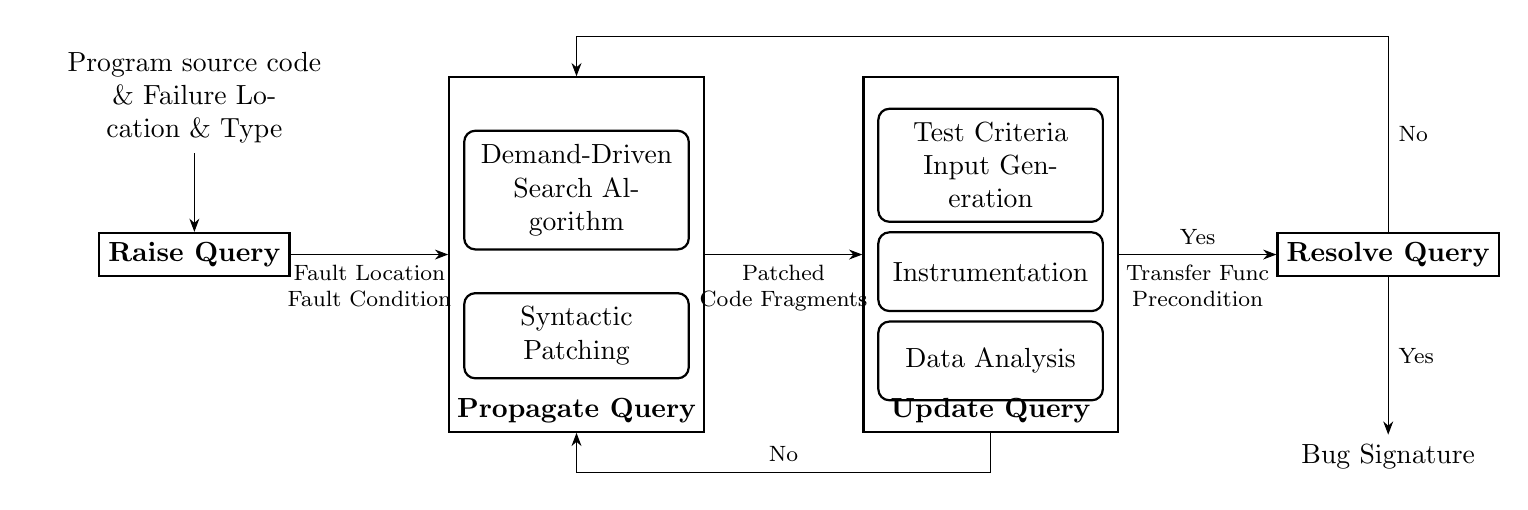
\begin{tikzpicture}[-Stealth,
      lab/.style={font=\footnotesize},
      every matrix/.style={minimum height=45mm,
        % fill=yellow!70!black,
        draw,
      },
      every node/.style={thick}
      ]
    \node (b1) [draw, font=\bf, thick] {Raise Query};

    \matrix (b2) [right=2cm of b1, draw,
      row sep=15pt,
      every node/.style={
        text width=2.5cm,
        % thin,
      },
      inner sep=0.5em,
      "Propagate Query" {below, anchor=south, font=\bf}
      ] {
      \node [align=center,
        draw, rounded corners,
        minimum height=10mm,
        ] {Demand-Driven\\ Search Algorithm};\\
      \node [align=center,
        draw, rounded corners,
        minimum height=10mm,] {Syntactic Patching};\\
      % \node [align=center, minimum height=10mm] {Propagate Query};\\
    };

    \matrix (b3) [right=2cm of b2,
      draw,
      every node/.style={
        text width=2.5cm,
        align=center
      },
      row sep=3pt,
      inner sep=0.5em,
      "Update Query" {below, anchor=south, font=\bf}
      ] {
      \node [draw,
        rounded corners, minimum height=10mm
        ] {Test Criteria\\Input Generation};\\
      \node [draw, rounded corners, minimum height=10mm] {Instrumentation};\\
      \node [draw, rounded corners, minimum height=10mm] {Data Analysis};\\
      % \node {Update Query};\\
    };

    
    \node (b4) [right=2cm of b3, draw, font=\bf] {Resolve Query};

    \node (in) [above=of b1, text width=4cm, align=center] {Program source code\\
      \& Failure Location \& Type};
    \node (out) [below=2cm of b4] {Bug Signature};

    \draw (in) --
    (b1);
    \draw (b1) --
    node [lab, below, align=center] {Fault Location\\Fault Condition}
    (b2);
    
    \draw (b2) --
    node [lab, below, align=center] {Patched\\ Code Fragments}
    (b3);

    \draw (b3) --
    node [lab, above] {Yes}
    node [lab, below, align=center] {Transfer Func\\ Precondition}
    (b4);
    \draw (b4) -- node [right, lab] {Yes} (out);

    \node (botline) at ([yshift=-5mm] b2.south) {};
    \draw (b3) --  (b3.south |- botline) --
    node [above, lab] {No}
    (botline.base) -- (b2);

    \node (topline) at ([yshift=5mm] b2.north) {};
    
    \draw (b4) --
    node [right, lab] {No}
    (b4.north |- topline) -- (topline.base) -- (b2);
  \end{tikzpicture}
  \caption{Demand-driven Dynamic Analysis Workflow}
\end{figure*}


\end{document}
